\documentclass{thesis-peach}

\thesistitle{Catchy Titles Are Good: But Avoid Being Cute}
\thesisauthor{Jacob O. Wobbrock}

\begin{acronym}
    \acro{HCI}{Human-Computer Interaction}
    \acro{PEACH}{Programming, Education, and Computer-Human Interaction}
    \acro{CS}{Computer Science}
\end{acronym}

\newcommand{\sysname}{Created Thing}

\abstract{
    The most important rule of Abstracts is that they describe the work, not the paper. 
Include, at most, one sentence of motivation. 
Save the rest of your motivation for the
Introduction. Effective Abstracts focus on two things: (1) Describing what was \emph{done}. (2) Describing what was \emph{found} (key results). 
Be specific about your key findings. 
Instead of \say{many} say \say{84\%}. 
Keep the Abstract to one paragraph and
fewer than 200 words.
}

\acknowledgment{
    This template is designed for students collaborating with the \ac{PEACH} Lab on their thesis projects.\footnote{April: If you use GPT products to help you write any part of the thesis, you should acknowledge its role.}
We would like to acknowledge that this template uses contents from the paper \say{Catchy titles are good: But avoid being cute}\footnote{https://faculty.washington.edu/wobbrock/pubs/Wobbrock-2015.pdf} from professor Jacob O. Wobbrock, the University of Washington.
}

\begin{document}

\section{Introduction}
The Introduction delivers the motivation for your paper. 
It explains \emph{why} you did the work you did. 
This is the primary function of the Introduction.
I have found a 5-point structure for Introductions to be particularly effective. (Here, I build on advice I received as
a Ph.D. student from Prof. Scott E. Hudson.)

\begin{itemize}
    \item State of the world…
    \item The big BUT...
    \item Therefore, we did...
    \item The key findings are...
    \item The contributions of this work are...
\end{itemize}

The state of the world is a description of issues in whatever \say{world} is relevant to your topic. 
Drawing on popular press can be effective here if recent news items or data from articles support your cause.

The big BUT is where a problem is introduced.
Or, similarly, a problem can be framed as an opportunity. 
Whether you are solving a problem or seizing an opportunity, motivate your work by connecting it to \emph{things that matter to people}.

One of the worst ways to motivate your work is using the \say{absence from the literature} argument. 
\say{Studies to date have
not …,} or \say{The literature is thus far silent on…,} or \say{Researchers have not yet examined how…} 
Such sentences are fine to add \emph{after} you have established a problem or opportunity worthy of pursuit in its own right. 
But as standalone motivational statements, absence-from-the-literature does not zing. 
Maybe the literature is silent on an issue
because that issue is not important.

After the big BUT, you will describe what you did, now in a bit more detail than in the Abstract. 
Devoting a paragraph to what you did is reasonable in the Introduction.

After saying what you did, you should offer the key results of what you did. 
What were the major findings? 
Whereas the Abstract might have devoted a sentence or two to key results, now you can devote a whole paragraph.

Finally, a good way to end your Introduction is by framing the contributions that your work makes. (See \say{Seven Research Contributions in HCI}\cite{wobbrock2012seven} for examples of different research contributions.) 
I often structure my contributions as a numbered list within a paragraph.
\say{The main contributions of this work are: (1) …; (2) …; (3) …}
(Most papers will have one to three contributions. 
Work that claims to have more than three contributions is often overstating how many contributions it makes.)

By structuring your Introduction with the 5-point outline, you succinctly motivate the work against a real problem or opportunity, and hook the reader by enticing them with the key results and contributions. 
They will want to know more.

Often, reviewers’ judgments about a piece are formed pretty quickly after reading the Introduction. 
If the Introduction reads poorly or is missing key aspects, that judgment can tilt negative very quickly.

Whatever expectations you set up in the Introduction, whatever research claims you make, you must deliver upon them in the rest of the paper. 
Over-claiming is a sure way to
get your paper rejected.

Do not make the main implication of your research that more research is needed. 
(It can be an implication, but not the main one, and certainly not the one called out at the end of the Introduction, Abstract, or Conclusion.) 
An Introduction (or Abstract or Conclusion) that ends with, “This work opens up new directions for further research into X” as its main answer to “so what?” is weak and uninspiring. 
What such a statement essentially means is that the chief benefit of your research is just more research. 
And apparently that research is left for others to do because, for some reason, you stopped short of doing it. 
Instead, make the main implication of your work that the problem or opportunity you set out to address is now at least somewhat addressed. 
\say{This work paves the way for more women to be better incorporated into software
development teams.} 
\say{This work opens up new directions in the development of assistive technology by using adaptive
user interfaces.} 
\say{This work lessens the challenges faced by single mothers as they try to incorporate educational technologies into their children’s lives.} 
The point is, the outcome of your research can’t just be more research, or why didn’t you do it and gain an actual solution to report?

In a 10-page paper, it is okay if the Introduction goes a bit onto the second page. 
In a 4-page paper, the Introduction should probably end somewhere on the first page.\footnote{April: Your final thesis report should range between 5 to 10 pages in length. It should not encompass every detail of your work but rather summarize and present it concisely.}

\begin{figure}
    \centering
    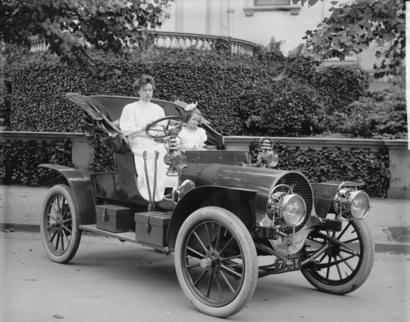
\includegraphics{figures/sample-franklin.png}
    \caption{Caption}
    \label{fig:enter-label}
\end{figure}
\section{Related Work}
The primary function of Related Work is to answer the following four questions: 
\begin{itemize}
    \item Who else has done work with relevance to this work of yours? \footnote{This can be a research paper, an open-source project, or a commercial product.}
    \item What did they do?
    \item What did they find?
    \item And how is your work here different?
\end{itemize}

This last step is called \emph{differentiation}.

(Sidebar: You will find that well-written Abstracts in others’ papers answer \say{What was done?} and \say{What was found?} and are immensely valuable to you as you scour the literature. 
In contrast, Abstracts that are mostly motivation or describe their paper, not their work, require you to look into the paper itself to have any idea what was actually done.
Such Abstracts are very unhelpful, but sadly, exceedingly common.)

Related Work should not read like a laundry list of who--did--what.
Related Work should offer insights and education
about prior work.
It should \emph{teach} readers something and help them understand the prior work better than they did before.

Skillfully written Related Work sections will often group prior work into themes. 
In 10-page papers, these themes may be subsections. 
Differentiation of the current work from prior
work can then be achieved on a per-theme basis, rather than differentiating against every piece of prior work raised.

Differentiation should not be defensive. It is not required that the current work assert itself as \say{better} than prior work. 
That is for reviewers to decide. Rather, current work must be \emph{different} than prior work. 
It must ask a different question, use a different method or technique, be built on different technology, or have different results. 
(The one exception to differentiation in this way is a pure replication study, although even then, there are usually attempts to augment or supplement the methods used.)
\section{Design of Your Widget}
After Related Work, the next sections begin the description of your work: \emph{What was done?} 
If you are using design-driven research, you will often begin by describing what you created. 
If you have a \sysname{}, this section often takes 2--3 full pages to describe it in a 10-page paper. 
This section should include things like the goals for the \sysname{}, the principles underlying it, the optimizations you favored, the tradeoffs you faced, the rationale for the choices you made, the design or engineering process you went through, how and why the Created Thing works, how it is built, its most important properties, its appearance, its function, how and in what situations is it used, and what its limitations are. 
Basically, you are trying to give a full, replicable--by--an--expert account of what you created, your \sysname{}.

Figures and diagrams should be used liberally throughout this section to illustrate key points. 
I personally prefer figures to be inline and between paragraphs, inserted just after the paragraph that first refers to them. 
(The only exception to this is Figure \ref{fig:enter-label}.) 
That way, the reader encounters the figures \say{in the flow of reading,} rather than out of sequence and having to jump their eyes back and forth from the text to the figure.

\subsection{Subsections}
Subsections are almost always used in these sections. 
Near the end of the section it is often reasonable to have an Implementation Details subsection describing things like how many lines of code are in your \sysname{} (if the thing involves software), what programming language it was written in, what platform it runs on, and related. 
Such subsections are not particularly interesting but for technical readers, they can help to illuminate aspects of the innovation.
But the main focus of these write-ups should not be on fungible implementation details; focus instead on the ideas behind the innovation and the ways those ideas were
realized.

\subsubsection{Subsubsections}
Unless you absolutely must use them, avoid using subsubsections. 
Even the word \say{subsubsections} is
unpleasant to read, let alone what is in them. \footnote{April: I slightly disagree with this. If a subsubsection makes your paper clearer to read, go ahead and use it.}
\section{Method (But don't just name it ``Method'')}

Regardless of whether you are reporting on design-driven research or scientific research (meaning, whether or not you have the previous section describing a Created Thing or not), you will often have a method section describing the research method(s) by which you carried out your scientific work.

(There are exceptions to this structure, such as engineering--oriented papers that provide no empirical validation of the \sysname{} save the fact that they made the \sysname{} exist in the first place. 
So-called \say{existence proof} papers are
entirely legitimate; in such cases, most of those papers will be filled with descriptions of the \sysname{}, and any study of that thing will be analytical, not empirical. 
The Method section may therefore become instead an analytical assessment of the \sysname{}’s properties, rather than a description of any empirical methods.)

For papers containing empirical scientific accounts of some phenomenon, the research methods employed must be described carefully and in great detail. 
These research methods may be quantitative, qualitative, or mixed, and they should follow established norms in related fields such as psychology, sociology, or anthropology. 
The following subsections give method outlines for two common study types, quantitative laboratory experiments and qualitative field studies.

\subsection{Method Outline for Quantitative Laboratory Experiments}
If you are writing up your method for a quantitative laboratory experiment, a common structure found in many psychology articles is as follows:

\emph{Participants:} Describe how many participants took part, their genders, their mean age (M=32.3 years), their age variance (SD=6.2 years), and any other important characteristics. 
If any inclusion or exclusion criteria were used, report them.
The means by which participants were sampled and recruited should also be reported. 
If participants were compensated, say how. 
Give enough detail that a similar group of participants could be recruited in the future by an expert reader.

\emph{Apparatus:} Describe the experiment setup, including what equipment was used, how it was arranged, how the laboratory was set up, and so on. 
Also describe whatever software was running and the computer system it was running on, including the operating system and version, the hardware make and model, and anything else relevant to the particular technology used, e.g., frames per second for video recording.

\emph{Procedure:} Often the longest subsection within Method, the Procedure subsection should describe the process participants went through from their arrival to their departure from the lab. What tasks did they perform? In what order?
How many? What constituted a single “trial?” Enough detail should be provided that an expert reader could re-run the experiment if they were given the same participants and apparatus.

\emph{Design \& Analysis:} This subsection describes the experiment formally, using one paragraph to describe the experiment design in statistical terms, and one paragraph to describe the statistical analysis. 
An effective technique for experiments with multiple factors is to lay out the factors and their levels in a list. 
For example, we might write, \say{The experiment was a 3×2×2 within-subjects design with the following factors
and levels}:
\begin{quote}
\begin{itemize}
    \item \emph{Devices}: mouse, trackball, touchpad;
    \item \emph{Desk}: sitting desk, standing desk;
    \item \emph{Illumination}: lighted, darkness;
\end{itemize}    
\end{quote}

The analysis paragraph covers the formal statistical analysis approach used. 
For example, it might report: \say{We collected
148 data points for each of 16 participants, giving us 2368 data points in all. 
Twenty-two of these data points were removed due to sensor failures, resulting in 2346 viable data points for analysis.
The analysis was carried out with a repeated measures ANOVA using Bonferroni adjustments for post hoc comparisons and the Greenhouse-Geisser correction for violations of sphericity.}
As with other subsections, the test here is whether an expert reader could repeat the analysis with the description given.

\subsection{Method Outline for Qualitative Field Studies}
Another common type of study is the qualitative field study.
Typically, such studies are reported using a wider range of structures than for laboratory experiments. 
Nevertheless, there are certain essential methodological aspects to cover when reporting a qualitative field study. 
You can also seek best practices from sociological or anthropological societies and journals.

\emph{Participants}: Your method report should include coverage of the participants in the study. 
Depending on your study type and terminology preference, these may be informants, respondents, or just generally participants. A thick description of these participants is important, much more so than for the laboratory experiment. 
How did you gain access to the participants?
Where and who were they? 
What roles did they occupy in the setting you were in? 
These are just a few of the questions to address about your participants.

\emph{Theory}: Research built on theory may describe how the field study was designed in terms of the theoretical constructs underpinning it. 
Often, theory serves as an aid to decisionmaking when designing any kind of study, and that rationale can be invoked in the study description: 
Why were certain participants chosen and not others? 
Why was a particular field setting chosen? 
Why was a certain research method preferred? 
What does theory say about the phenomena being
studied and how it should be studied?

\emph{Procedures}: The procedures used in the field should also be described. 
These procedures may be about how the data were
gathered or recorded, how informants or settings were chosen and accessed, what questions were asked, what artifacts were gathered, what probes were used, how much time was spent with certain participants or at various sites, and where and how certain observations were made. 
Was an ethnographic account the goal? 
Was participant observation or non-participant observation used? How? 
The one type of procedure that is usually covered separately is the procedure for data analysis, which is next.

\emph{Analysis}: How were the qualitative data analyzed? 
How was objectivity and validity ensured? Many formal qualitative studies use grounded theory as an analysis method. 
If so, then the procedures that you followed for open coding, axial coding, selective coding, and theory formation should be
described in detail. 
Give a representative sample of your codes.
You could also give a link to an online version of a full coding manual. 
Was inter-rater reliability assessed?
How? 
And what was the outcome? 
Give enough detail that the analysis could be replicated by an expert reader if he or
she had your data.

\section{Results}
At last we reach the exciting part, your Results! 
Your Results section speaks for itself: report on the results of your work in an organized way. 
Refrain from reporting on the significance of these results until the Discussion section, which comes next. 
For now, report on the results dispassionately. 
Use charts, graphs, and tables as appropriate. 
Good Results sections do not simply jam a bunch of numbers in, but \say{tell a story with data,} creating an easy-to-read narrative flow that does not make the reader do too much work to figure out what happened.

For quantitative laboratory studies, often the Results section is divided into subsections by dependent variable, i.e., the things that were measured. 
When including the results of statistical tests, do not just say that there was a significant effect, interpret that effect for the reader. 
\begin{quote}
    Worse: \say{There was a significant main effect of Illumination on pointing time (F(1,28)=15.79, p<.0001).} 
\end{quote}
\begin{quote}
    Better: \say{There was a significant main effect of Illumination on pointing time (F(1,28)=15.79, p<.0001), as lighted conditions caused faster pointing than darkened conditions.}
\end{quote}

For qualitative field studies, often the Results section is divided into subsections around emergent themes. 
Results sections may be quite long, incorporating numerous observations and direct quotes from participants. 
Organizing your results in subsections is key to creating an easy--tofollow story.
\section{Discussion}
Whereas the Results section reported on what was \emph{found}, the Discussion section reports on what was \emph{interesting} and what \emph{matters}. 
Some questions to consider when writing your Discussion section: 
What are the implications of your results?
What do they mean for this topic and your field?
What is important and worthy of again being called to the reader’s attention? 
What was surprising? unexpected? intriguing? 
Did you fulfill the promises you set out in the Introduction via the claims you made about your work? 
Were any hypotheses confirmed or disconfirmed? 
Were the predictions of any theory upheld or refuted? 
What worked and what did not work? 
(This is a chance to be honest and show that you are objective with respect to your own work.)

The Discussion is not usually divided into subsections, but it can be if it is long. 
One subsection sometimes included at the end of Discussion sections is Limitations. 
In a single paragraph, lay out what the evident limitations of your study were and caution against faulty interpretations or overgeneralization of your results.
\section{Future Work}
What are the \say{big idea} next steps that follow from your work? 
Avoid merely incremental next steps that read like a TODO list. 
Instead, step back and reflect on the implications of the work and where they lead. 
What are the intellectual directions that should be taken on this topic? 
It is often better to offer one or two well-considered inspiring next steps than a laundry list of smaller items.
\section{Conclusion (Not Conclusion{\color{red}s})}
Your Conclusion is the section in which you: 
(1) affirm that you have delivered on the claims made in your Introduction,
(2) summarize the contributions of the work, 
(3) make any key points with which you would like to leave the reader, and
(4) point to a bright future, a better world, for your work having been done in it.
It should not be necessary to re-report the key findings of the work, although doing so to a limited extent can be okay. 
The findings have already been reported, so it is better to \say{zoom out} and report on the key contributions of the work.
\begin{quote}
    Worse: \say{We showed in this work that illuminated office conditions result in an 84\% improvement in pointing speed than dark offices.}
\end{quote}
\begin{quote}
    Better: \say{This work contributed the first empirical study of pointing under different office illumination conditions.}
\end{quote}
\begin{quote}
    Unnecessary: \say{This work contributed the first empirical study of pointing under different office illumination conditions, finding that illumination improves pointing speed by 84\% over dark offices.}
\end{quote}
    
Try to frame the contributions of the work such that they speak to your broader scholarly community, not just those interested in your narrow topic. 
Imagine someone from the popular press reading your Conclusion. 
Could they imagine a news story on your work from what they read?

Now that you have been given numerous tips on how to structure your research paper, I am confident that you will do right by the good research you are doing by writing it in ways that others can understand and appreciate. 
The world will be made better for all the work you do and the way you communicate it. 
Go forth and write well!


%%
%% If your work has an appendix, this is the place to put it.
\appendix

\section{Common Elements}

\subsection{Tables}

The ``\verb|acmart|'' document class includes the ``\verb|booktabs|''
package --- \url{https://ctan.org/pkg/booktabs} --- for preparing
high-quality tables.

Table captions are placed {\itshape above} the table.

Because tables cannot be split across pages, the best placement for
them is typically the top of the page nearest their initial cite.  To
ensure this proper ``floating'' placement of tables, use the
environment \textbf{table} to enclose the table's contents and the
table caption.  The contents of the table itself must go in the
\textbf{tabular} environment, to be aligned properly in rows and
columns, with the desired horizontal and vertical rules.  Again,
detailed instructions on \textbf{tabular} material are found in the
\textit{\LaTeX\ User's Guide}.

Immediately following this sentence is the point at which
Table~\ref{tab:freq} is included in the input file; compare the
placement of the table here with the table in the printed output of
this document.

\begin{table}[h]
  \caption{Frequency of Special Characters}
  \label{tab:freq}
  \centering
  \begin{tabular}{ccl}
    \toprule
    Non-English or Math&Frequency&Comments\\
    \midrule
    \O & 1 in 1,000& For Swedish names\\
    $\pi$ & 1 in 5& Common in math\\
    \$ & 4 in 5 & Used in business\\
    $\Psi^2_1$ & 1 in 40,000& Unexplained usage\\
  \bottomrule
\end{tabular}
\end{table}

To set a wider table, which takes up the whole width of the page's
live area, use the environment \textbf{table*} to enclose the table's
contents and the table caption.  As with a single-column table, this
wide table will ``float'' to a location deemed more
desirable. Immediately following this sentence is the point at which
Table~\ref{tab:commands} is included in the input file; again, it is
instructive to compare the placement of the table here with the table
in the printed output of this document.

\begin{table*}
  \caption{Some Typical Commands}
  \label{tab:commands}
  \centering
  \begin{tabular}{ccl}
    \toprule
    Command &A Number & Comments\\
    \midrule
    \texttt{{\char'134}author} & 100& Author \\
    \texttt{{\char'134}table}& 300 & For tables\\
    \texttt{{\char'134}table*}& 400& For wider tables\\
    \bottomrule
  \end{tabular}
\end{table*}

Always use midrule to separate table header rows from data rows, and
use it only for this purpose. This enables assistive technologies to
recognise table headers and support their users in navigating tables
more easily.

\subsection{Math Equations}
You may want to display math equations in three distinct styles:
inline, numbered or non-numbered display.  Each of the three are
discussed in the next sections.

\subsubsection{Inline (In-text) Equations}
A formula that appears in the running text is called an inline or
in-text formula.  It is produced by the \textbf{math} environment,
which can be invoked with the usual
\texttt{{\char'134}begin\,\ldots{\char'134}end} construction or with
the short form \texttt{\$\,\ldots\$}. You can use any of the symbols
and structures, from $\alpha$ to $\omega$, available in
\LaTeX~\cite{Lamport:LaTeX}; this section will simply show a few
examples of in-text equations in context. Notice how this equation:
\begin{math}
  \lim_{n\rightarrow \infty}x=0
\end{math},
set here in in-line math style, looks slightly different when
set in display style.  (See next section).

\subsubsection{Display Equations}
A numbered display equation---one set off by vertical space from the
text and centered horizontally---is produced by the \textbf{equation}
environment. An unnumbered display equation is produced by the
\textbf{displaymath} environment.

Again, in either environment, you can use any of the symbols and
structures available in \LaTeX\@; this section will just give a couple
of examples of display equations in context.  First, consider the
equation, shown as an inline equation above:
\begin{equation}
  \lim_{n\rightarrow \infty}x=0
\end{equation}
Notice how it is formatted somewhat differently in
the \textbf{displaymath}
environment.  Now, we'll enter an unnumbered equation:
\begin{displaymath}
  \sum_{i=0}^{\infty} x + 1
\end{displaymath}
and follow it with another numbered equation:
\begin{equation}
  \sum_{i=0}^{\infty}x_i=\int_{0}^{\pi+2} f
\end{equation}
just to demonstrate \LaTeX's able handling of numbering.

\subsection{Figures}

The ``\verb|figure|'' environment should be used for figures. One or
more images can be placed within a figure. If your figure contains
third-party material, you must clearly identify it as such, as shown
in the example below.
\begin{figure}[h]
  \centering
  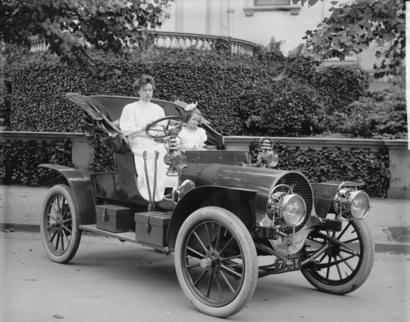
\includegraphics[width=\linewidth]{figures/sample-franklin.png}
  \caption{1907 Franklin Model D roadster. Photograph by Harris \&
    Ewing, Inc. [Public domain], via Wikimedia
    Commons. (\url{https://goo.gl/VLCRBB}).}
  \Description{A woman and a girl in white dresses sit in an open car.}
\end{figure}

Your figures should contain a caption which describes the figure to
the reader.

Figure captions are placed {\itshape below} the figure.

Every figure should also have a figure description unless it is purely
decorative. These descriptions convey what’s in the image to someone
who cannot see it. They are also used by search engine crawlers for
indexing images, and when images cannot be loaded.

A figure description must be unformatted plain text less than 2000
characters long (including spaces).  {\bfseries Figure descriptions
  should not repeat the figure caption – their purpose is to capture
  important information that is not already provided in the caption or
  the main text of the paper.} For figures that convey important and
complex new information, a short text description may not be
adequate. More complex alternative descriptions can be placed in an
appendix and referenced in a short figure description. For example,
provide a data table capturing the information in a bar chart, or a
structured list representing a graph.  For additional information
regarding how best to write figure descriptions and why doing this is
so important, please see
\url{https://www.acm.org/publications/taps/describing-figures/}.

\subsection{Code Snippet}

\begin{minted}[frame=single,framesep=10pt]{python}
# main notebook
foo = 123
\end{minted}
\begin{minted}[frame=single,framesep=10pt]{python}
# parallel cell group named 'plel'
foo = foo +  5
bar = 'hello'
foo # note: in "standard" Jupyter, this line outputs '128' when the user executes this cell
\end{minted}



%%
%% The next two lines define the bibliography style to be used, and
%% the bibliography file.
\bibliographystyle{ACM-Reference-Format}
\bibliography{references}

\end{document}
